\documentclass{article}
\usepackage[UTF8]{ctex}
\usepackage{geometry}
\usepackage{multirow}
\usepackage{natbib}
\geometry{left=3.18cm,right=3.18cm,top=2.54cm,bottom=2.54cm}
\usepackage{graphicx}
\pagestyle{plain}	
\usepackage{setspace}
\usepackage{enumerate}
\usepackage{caption2}
\usepackage{datetime} %日期
\renewcommand{\today}{\number\year 年 \number\month 月 \number\day 日}
\renewcommand{\captionlabelfont}{\small}
\renewcommand{\captionfont}{\small}
\begin{document}

\begin{figure}
    \centering
    
\includegraphics[width=8cm]{upc.png}

    \label{figupc}
\end{figure}

	\begin{center}
		\quad \\
		\quad \\
		\heiti \fontsize{45}{17} \quad \quad \quad 
		\vskip 1.5cm
		\heiti \zihao{2} 《计算科学导论》个人职业规划
	\end{center}
	\vskip 2.0cm
		
	\begin{quotation}
% 	\begin{center}
		\doublespacing
		
        \zihao{4}\par\setlength\parindent{7em}
		\quad 

		学生姓名:\underline{\qquad  周时 \qquad \qquad}

		学\hspace{0.61cm} 号:\underline{\qquad 1907010118\qquad}
		
		专业班级:\underline{\qquad 计科1901 \qquad  }
		
        学\hspace{0.61cm} 院:\underline{计算机科学与技术学院}
% 	\end{center}
		\vskip 1.5cm
		\centering
		\begin{table}[h]
            \centering 
            \zihao{4}
            \begin{tabular}{|c|c|c|c|c|c|c|c|c|}
            % 这里的rl 与表格对应可以看到,姓名是r,右对齐的;学号是l,左对齐的;若想居中,使用c关键字。
                \hline
                \multicolumn{5}{|c|}{分项评价} &\multicolumn{2}{c|}{整体评价}  & 总    分 & 评 阅 教 师\\
                \hline
                自我 & 环境 & 职业 & 实施 & 评估与 & 完整性 & 可行性 &\multirow{2}*{} &\multirow{2}*{}\\
                分析& 分析& 定位 & 方案 & 调整 & 20\% & 20\% & ~&~ \\\            
                10\% & 10\% & 15\% & 15\% & 10\% & &  &~ &~\\
                \cline{1-7} 
                & & & & & & & ~&~ \\
                & & & & & & & ~&~ \\
                \hline      
            \end{tabular}
        \end{table}
		\vskip 2cm
		\today
	\end{quotation}

\thispagestyle{empty}
\newpage
\setcounter{page}{1}
% 在这之前是封面,在这之后是正文
\section{自我分析}
	自我分析即对自己进行全方位、多角度的分析,目的是认识自己、了解自己。只有认识了自己,才能对自己的职业做出正确的选择,才能选定适合自己发展的职业生涯路线,才能对自己的职业生涯目标做出最佳抉择。\par
	自我分析包括:\par
\subsection{自然条件}
男,18周岁,身体条件良好,健康状况良好,现居住在山东省青岛市黄岛区中国石油大学(华东) 13号公寓。\par
\subsection{性格分析}
乐观主义,团队合作能力较强,自控力较差,待人温和,尽量避免与任何人出现矛盾,善于学习和接受新的事物,对自己难以改变或无法改变的不满现实自怨自艾,对新奇的科技数码产品非常感兴趣,价值观整体比较激进和偏向自由主义。\par
\subsection{教育与学习经历}
毕业于吉林省通榆县第一中学,通过普通高等学校全国统一考试进入我校。\par
\subsection{工作与社会阅历}
曾经帮助家属务农及畜牧。\par
\subsection{知识、技能与经验}
基本的程序设计语言(c++)知识,基本的离散数学与高中数学知识,以及夯实的义务教育基础。
基本的office办公组件的使用。
\par
\subsection{兴趣爱好与特长}
爱好数码设备体验,购买,喜欢鼓捣一些新奇的技术给安卓手机刷ROM及iOS 系统越狱,windows重装系统。会唱歌,古典音乐的鉴赏以及电子音乐的制作。关注股市动态与行情,观察总结市场的规律。\par
\section{环境分析}
环境分析主要是评估周边各种环境因素对自己职业生涯发展的影响。每一个人都处在一定的环境之中,职业发展必然要受到所处环境的影响,只有充分了解和把握所处环境的现状、特点、发展变化趋势,才能做到在复杂的环境中避害趋利,使你的职业生涯规划具有实际意义。\par
环境分析包括:\par
\subsection{社会环境分析}
我国正处于全面建成小康社会的关键时期,需要大量中国技术人的努力,而我国的相关政策也对此大力扶持,对人工智能等领域政策扶持力度加大,政治形势对我未来的发展十分有利。
近年来5G、人工智能、大数据、区块链等科技热词频频爆红网络,科技股及科技相关的基金涨幅较大(如:前开源人工智能聚合、鹏华中证信息指数),科技行业正在快速聚集资本,未来形势较好。
随着IT行业的火爆,大量人才涌入IT行业,以及大量IT技术培训班的出现(如北大青鸟)使得IT行业人才量剧增,但就目前来看,高精尖人才仍供不应求,只是具有基本编程能力的技术型人才不再受到欢迎甚至数量过饱和。只有强化自己的能力,提高自己的不可替代性,才能加大自己的竞争力,就目前来看IT行业薪资很高但是就业压力较大。
\par
\subsection{家庭环境分析}
未婚,经济未能独立,需父母提供生活费,家人期望自己能够在稳定的事业单位找到稳定的工作,或从事学术研究,造福社会,但与本人意愿不符。父亲是白求恩医科大学毕业的放射科医师,母亲是中专毕业的小学语文教师,父辈由山东闯关东来到东北,家族规模较小,故无特定传统。\par
\subsection{职业环境分析}
①互联网用户规模及普及率不断提高\par
		截止至2018年底,我国网民规模达到8.29亿,全年新增网民5653万,互联网普及率达61.2\%(数据源自中国互联网络信息中心(CNNIC)在京发布第44次《中国互联网络发展状况统计报告》),互联网正在或已经成为我们生活中不可或缺的财富\par
②互联网基础资源日益丰富\par
		2019年是阿帕网诞生50周年,也是中国全功能接入国际互联网25周年。25年间,中国已发展成为一个网络大国,互联网用户规模连续多年稳居世界第一,“.CN”保有量近三年在国家和地区域名中保持全球第一,互联网新应用、新业态、新模式层出不穷。(参考资料首届中国互联网基础资源大会在京举行)\par
③互联网应用领域不断拓展\par
		首先在衣食住行、健康医疗、通讯、搜索和金融服务等方面日趋完善,而且在更多领域逐渐拓展,未来发展前景宽广。\par
\subsubsection{目标职业}
	本人想要成为一名算法工程师,图1是腾讯公司对算法工程师的要求个人觉得很具有代表性。\par
\begin{figure}[h!]
\centering
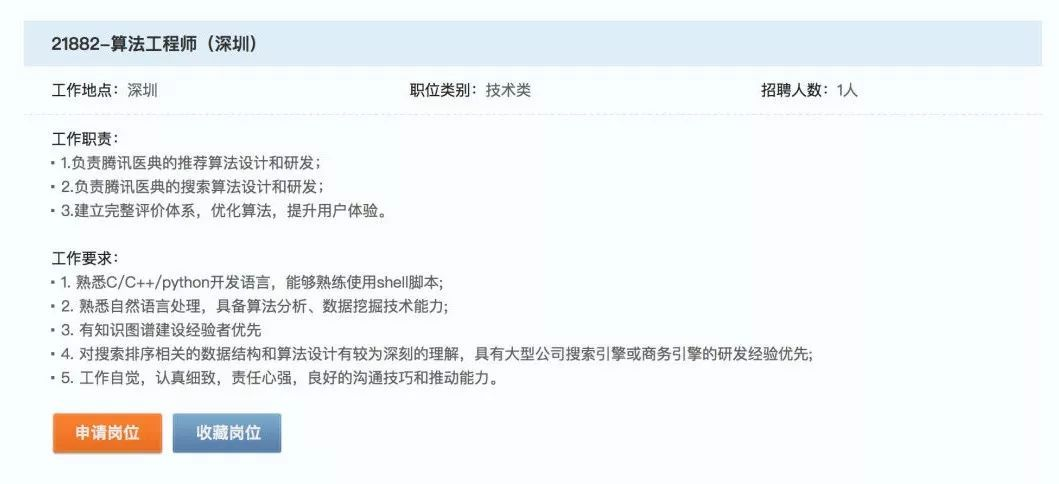
\includegraphics[scale=0.6]{1}
\caption{图一:腾讯公司招聘启事}
\label{fig:1}
\end{figure}

从图片中我们可以看到,想要成为一名优秀的算法工程师,单单只精通一种语言或技术是不够的,需要多维度,全方面的能力,并且对数据分析要有很高的造诣。\par

\subsection{地域与人际环境分析}

工 作城市的气候水土、文化特点、发展前景;人脉与人际关系等。\par
\par 
\subsubsection{深圳的气候特点}

深圳市位于广东省中南沿海地区,珠江入海口之东偏北,所处纬度较低,属亚热带海洋性气候。由于深受季风的影响,夏季盛行偏东南风,时有季风低压、热带气旋光顾,高温多雨;其余季节盛行东北季风,天气较为干燥,气候温和,年平均气温22摄氏度,雨量充足,每年4~9月为雨季,降雨量较多。

\subsubsection{深圳的文化特点}
深圳特区的文化是,具有移民文化、窗口文化、引桥文化、多元文化及市民的开放型文化特点。从建设深圳经济特区的意义来看,特区文化应具有超前性、商品性与兼容性,既能满足特区市民不同层次的文化需求,又能为港澳台同胞及海外华人所能接受的开放、兼容、多元的新型文化。
\subsubsection{深圳的发展前景}
1.深圳地区年龄结构在北上广深四大城市中是最为年轻的,这也是未来深圳继续保持高速发展的最重要的前提保障。从统计数据上看,深圳常住人口平均年龄为32.5岁属于全国人口最年轻的城市青年人才的不断流入,成为支撑深圳未来发展的最有利前提条件。

\begin{figure}[h!]
\centering
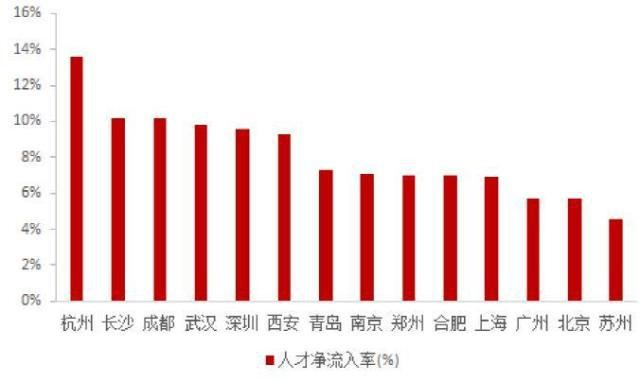
\includegraphics[scale=0.5]{2}
\caption{ 图二:2017年深圳人才净流入率 }
\label{fig:2}
\end{figure}

2.深圳在城市对企业的吸引力和企业在城市的发展力两方面均居于全国首位,企业经营环境较为有利。

\begin{figure}[h!]
\centering
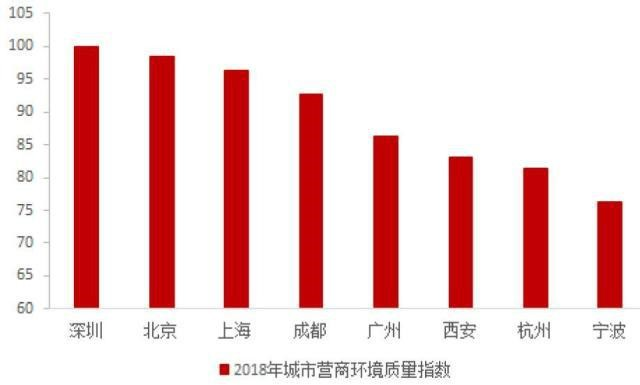
\includegraphics[scale=0.5]{3}
\caption{  图三:深圳地区营商环境相对较好 }
\label{fig:3}
\end{figure}
3.深圳的新兴产业发展势头强劲,深圳地区第三产业特别是信息技术服务业在GDP中的占比明显高于全国平均水平,产业结构相对较为先进。

\begin{figure}[h!]
\centering
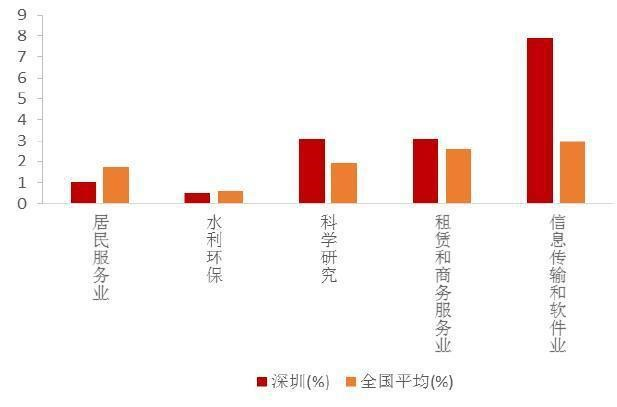
\includegraphics[scale=0.5]{4}
\caption{ 图四:深圳信息产业占比较高(截至2017年末) }
\label{fig:4}
\end{figure}
\par
\subsubsection{城市人脉}
有父亲的同学在华为任职。\par



\section{职业定位}
在准确地对自己和环境做出了分析之后,确定适合自己行业和有实现可能的职业发展目标。职业定位时要注意与自己的自然条件、知识背景、技能特长、性格特点、兴趣爱好是否匹配,考虑与自己所处的环境是否相适应。职业定位决定了职业发展中的行为和结果,是制定职业生涯规划的关键,应当科学合理,具有可行性。\par
职业定位包括:\par

\subsection{行业领域定位与理由}
我对我自己未来所处行业的定位是:IT行业\par
理由:算法工程师是IT行业从业人员


\subsection{职业目标与可行性分析}
\par
成果目标、经济目标、能力目标、职务目标等。\par 
\begin{enumerate}[(1)]
	\item 短期目标(大学4年)\par
     学会算法工程师的基础能力,包括:
\begin{itemize}
    \item Python、C++、Java这类编程语言,这三种也是算法工程师需要了解的主流编程语言,一般掌握其一就够,看不同公司。
    \item Sql,Sql也是一门编程语言。大数据场景下,要了解Hive Sql。
    \item Sklearn
    \item Tensorflow
    \item Spark ML
\end{itemize}
	\item 中长期目标(5-10年)。\par
 	取得算法工程师的核心能力,和一些辅助性的的技术能力,包括:
\begin{itemize}
    \item Pipeline 构建能力
    \item 数据分析能力
\end{itemize}
	经济,职务目标:
\begin{itemize}
    \item 毕业后5年内薪酬达到30万。
    \item 毕业后5年内达到p7级别
\end{itemize}	

	
\end{enumerate}




\section{实施方案}
\begin{enumerate}[1、]
	\item 利用现有条件和自身优势以实现职业生涯目标。
\begin{itemize}
    \item 利用自己对技术的渴望与好奇心充实自己的技术库
    \item 努力训练算法,争取成为我校ACM俱乐部现役队员
\end{itemize}
	\item 克服缺点、弥补不足、增长知识、提高能力以实现职业生涯目标。
	\item 处理人际关系和发展人脉以实现职业生涯目标。
	\item 处理工作与家庭、生活的关系以实现职业生涯目标。
\begin{itemize}
    \item 合理分配工作与生活的平衡
    \item 多抽出时间陪陪家人
\end{itemize}

	\item 处理释放工作压力、保证身心健康以实现职业生涯目标。
\begin{itemize}
   \item 保持规律的作息时间
    \item 合理安排工作学习与放松的时间,做到劳逸结合
    \item 适当出去旅游,出国,开拓眼界
\end{itemize}

\end{enumerate}
\par 

\section{评估与调整}
由于影响职业生涯规划的因素很多,且大都处于动态变化之中,因此职业生涯规划应定期评估,并根据影响因素的变化和实施结果的情况及时作出调整,这样才能保证其行之有效。\par 
\subsection{评估时间}
	一学年评估一次。
\subsection{评估内容}
评估下列目标是否达成:
\begin{itemize}
\item 成果目标
\item 经济目标
\item 能力目标
\item 职务目标
\end{itemize}	
	分析未达成原因,做出总结。


\end{document}
